


\section{Experiments}

In order to evaluate the effects of different components in SOVI and compare it with state-of-the-art approaches, we conduct series of experiments on two datasets, YouTubeVOS \cite{xu2018Youtube} and DAVIS \cite{davis_2017}.
%We test on two datasets, YouTubeVOS \cite{xu2018youtube} and DAVIS \cite{davis_2017}, to compare the proposed STSENet with state-of-the-art methods. %Several ablation studies are conducted to prove the effectiveness of spatial details and temporal information in video inpainting.
\subsection{Experimental Settings}
\textbf{Dataset.} 
YouTubeVOS and DAVIS are widely used for evaluation in recent video inpainting approaches.
YouTubeVOS is a large-scale dataset that contains 4,453 YouTube video clips. These videos are close to real-world scenarios
 with 70+ common objects. 
The videos are officially split into three parts, 3,471 for training, 474 for validating, and 508 for testing. 
DAVIS dataset is for video object segmentation containing 150 video clips, among which 60 randomly sampled clips are for testing of object removal. And the rest part is used for training.
The videos are complex with occlusions, fast motion, and various objects. 

\noindent \textbf{Mask Setting.} Considering various real-world applications, we test our method on four kinds of mask settings in this paper. 
They are different in shapes and positions of the missing regions.
\begin{enumerate}
	\item Fixed square mask. The size and position of the missing square region are fixed through the whole video. 
	\item Moving square mask. The position and size of the square mask change over frames. 
	\item Free-from mask. We apply irregular mask which imitates hand-drawn masks on each frame, following \cite{liu2018partialinpainting}. 
	\item Foreground object mask. This type of masks is defined to line out the foreground objects in videos, which is used for object removal.
\end{enumerate}


\noindent \textbf{Implementation Details.} 
In the data preparation stage, we randomly sample a clip every 40 frames from each video in the datasets.
The video frames are resized into $256\times256$.
%
The training process consists of three steps.
First, we  train the ENet and FNet jointly using Adam optimizer with $\beta=(0.9, 0.999)$.
The learning rate is set to $1e-4$ for $N^E$ and $G^F$ and $1e-5$ for $D^E$. Then, the TINet is trained with the learning rate of $1e-4$ for $G^I$, and $4e-4$ for $D^I$. Finally, we fix the former parts and train the temporal ensemble module with the learning rate of $1e-4$. We do not use weight decay in training.
As for the hyper-parameters, $\lambda_1=10.0,\lambda_2=5.0, \lambda_3=0.1$.

\noindent \textbf{Evaluation Metrics.} 
We use three commonly-used metrics to quantitatively evaluate the performance of our method. They are structural similarity index (SSIM) \cite{wang2004image}, peak signal-to-noise ratio (PSNR), and Fr{\'e}chet Inception Distance (FID) \cite{heusel2017gans}. 
Besides, the quantitative metrics can not be used in the experiments of foreground object removal, since there is no ground truth available. So we conduct a user study for video foreground object removal. 
%\cxj{Where these three metrics are used compared with object removal?}
%
%Besides, since there is no ground truth for the experiments of object removal, 



\begin{figure*}[t]
	\centering
	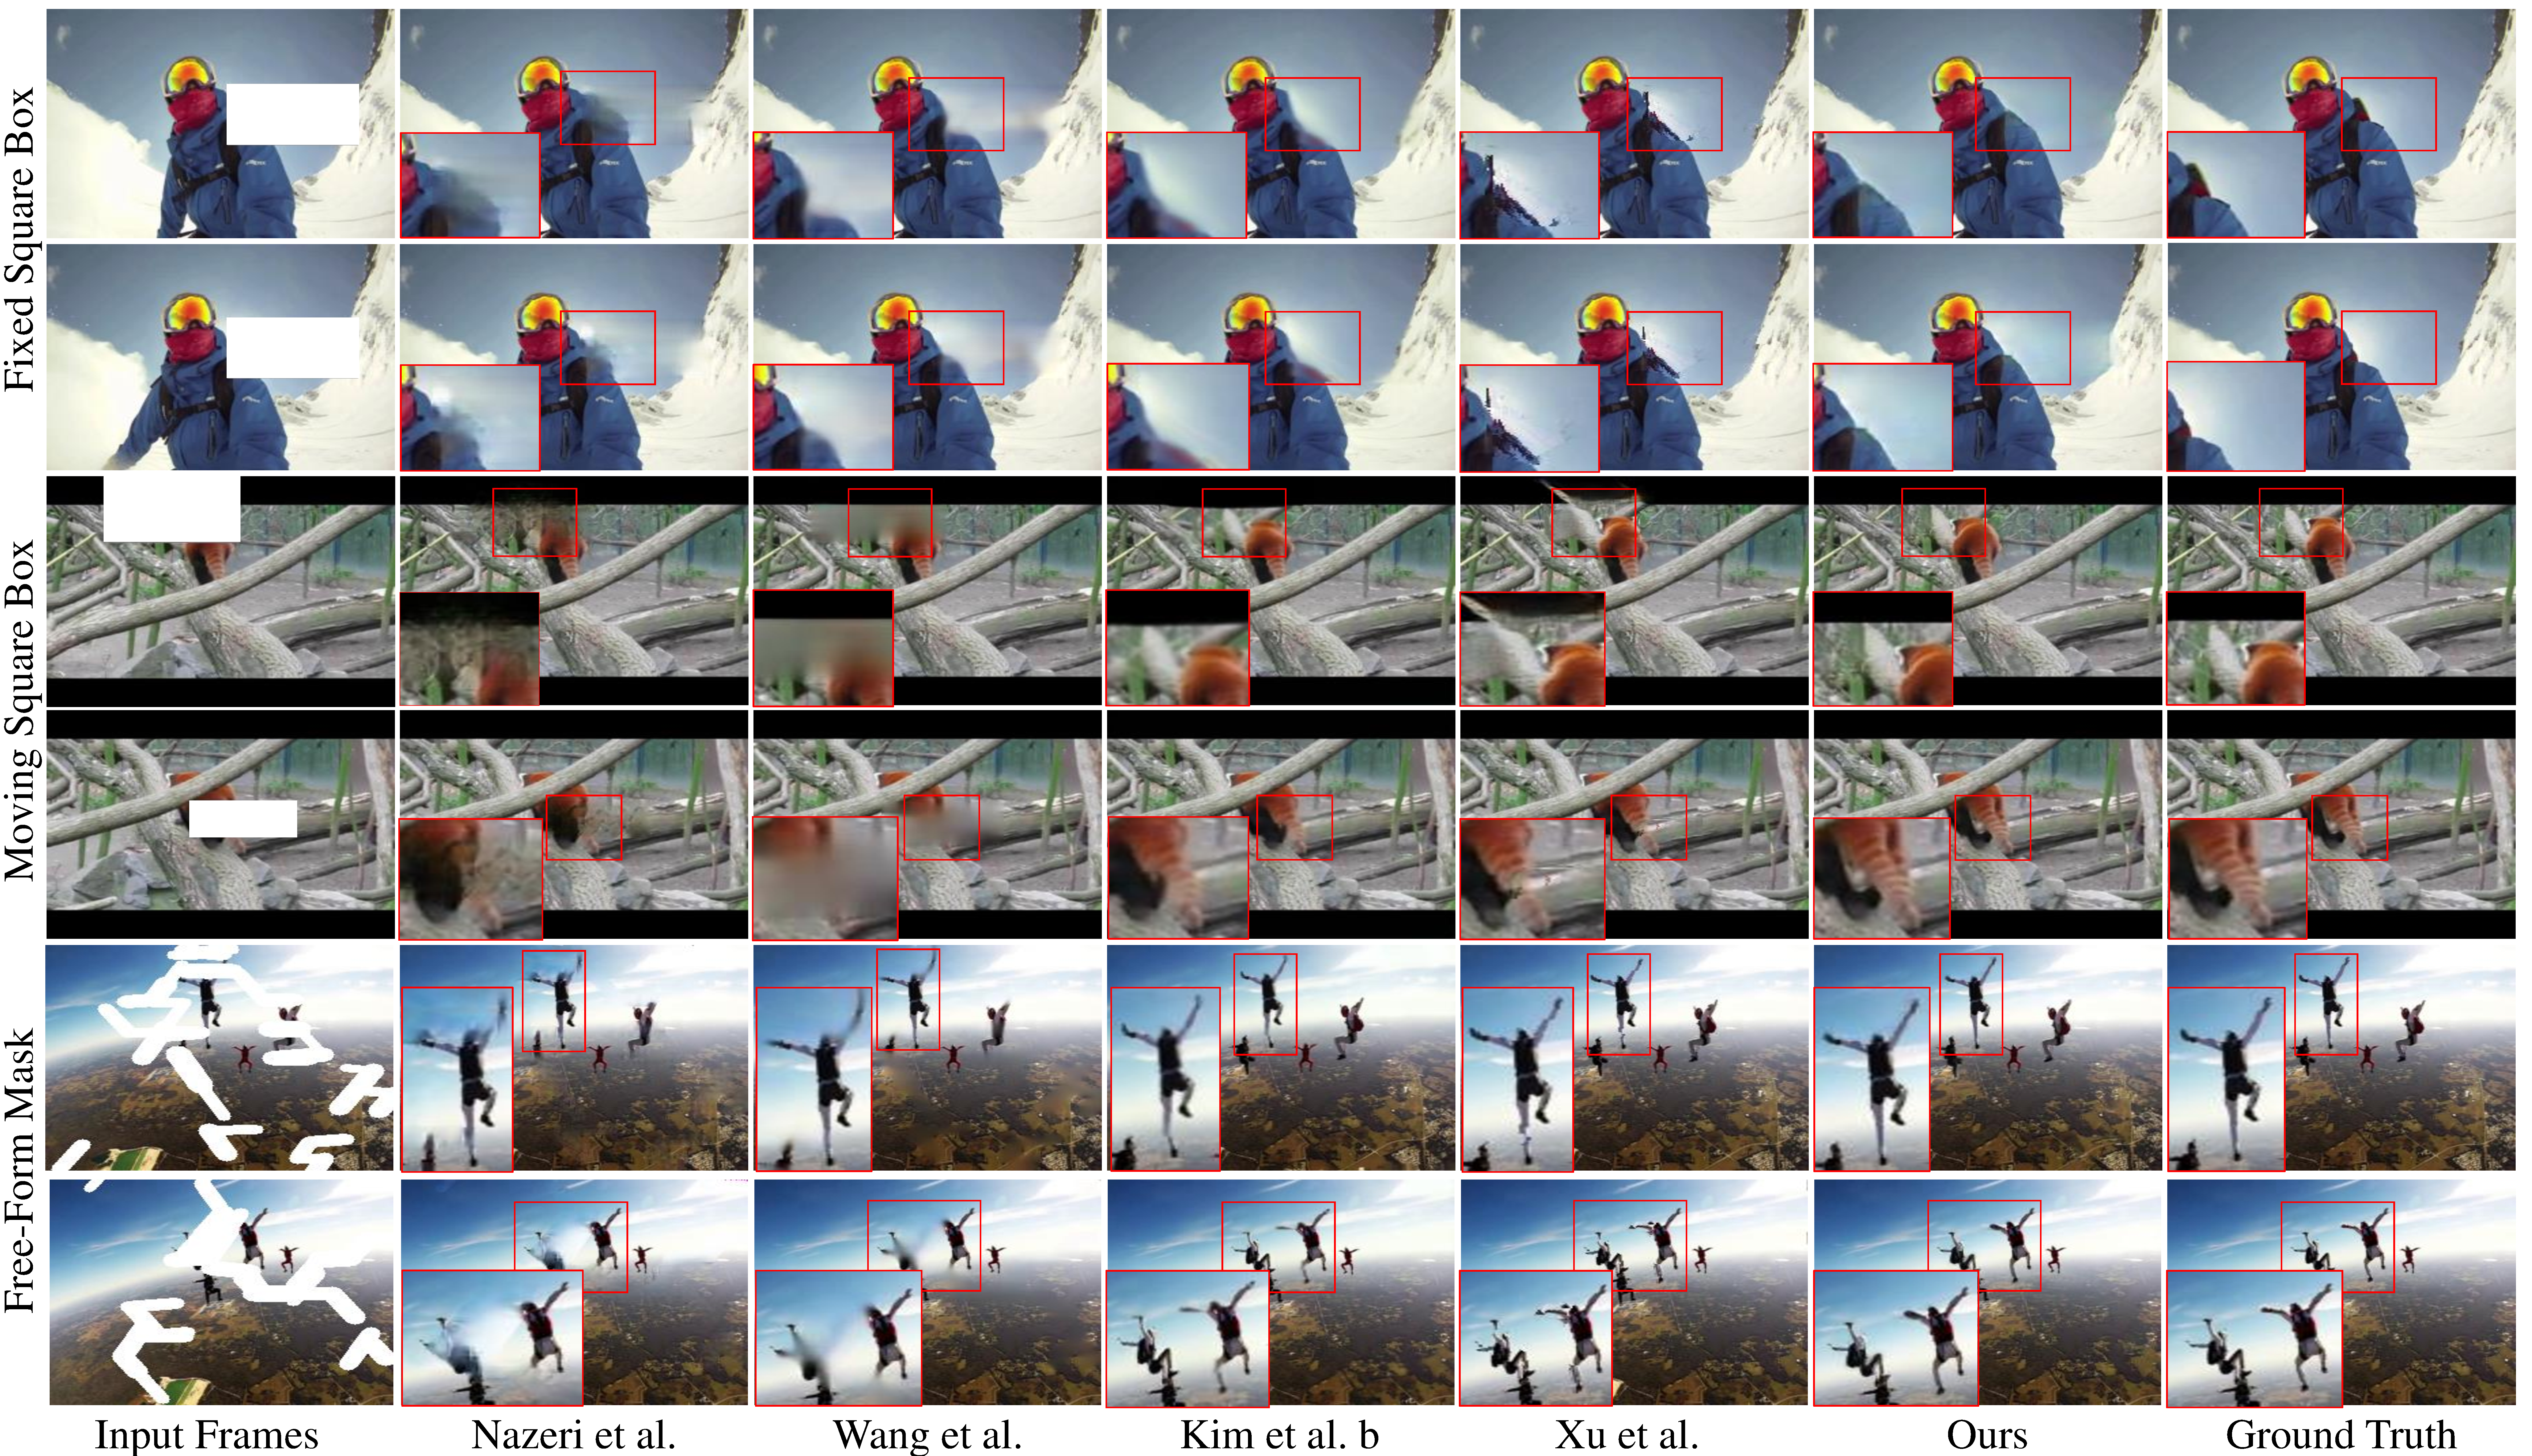
\includegraphics[scale=0.127]{viszong} % Reduce the figure size so that it is slightly narrower than the column. Don't use precise values for figure width.This setup will avoid overfull boxes. 
	\caption{Visualization for video inpainting on YouTubeVOS. Our method can produce frames with finer sturcture than existing methods. }
	\label{viszong}
\end{figure*}




\subsection{Ablation Study}
To demonstrate the effectiveness of proposed components in our method, we first conduct ablation study on YouTubeVOS. 

\subsubsection{Effect of Structure Clues in TINet.}



To evaluate the effects of structural information in video inpainting, we successively add different parts to the baseline and compare their performances. Three variants are used: 'STI', '+edge input', and '+SAM'. 
'STI' is the baseline using only texture inpainting network, without either structure clues or temporal information. '+edge input' is the model that uses the predicted edge maps as input. '+SAM' is the model to which structure attention module is applied.
\begin{figure}[!ht]
	\centering
	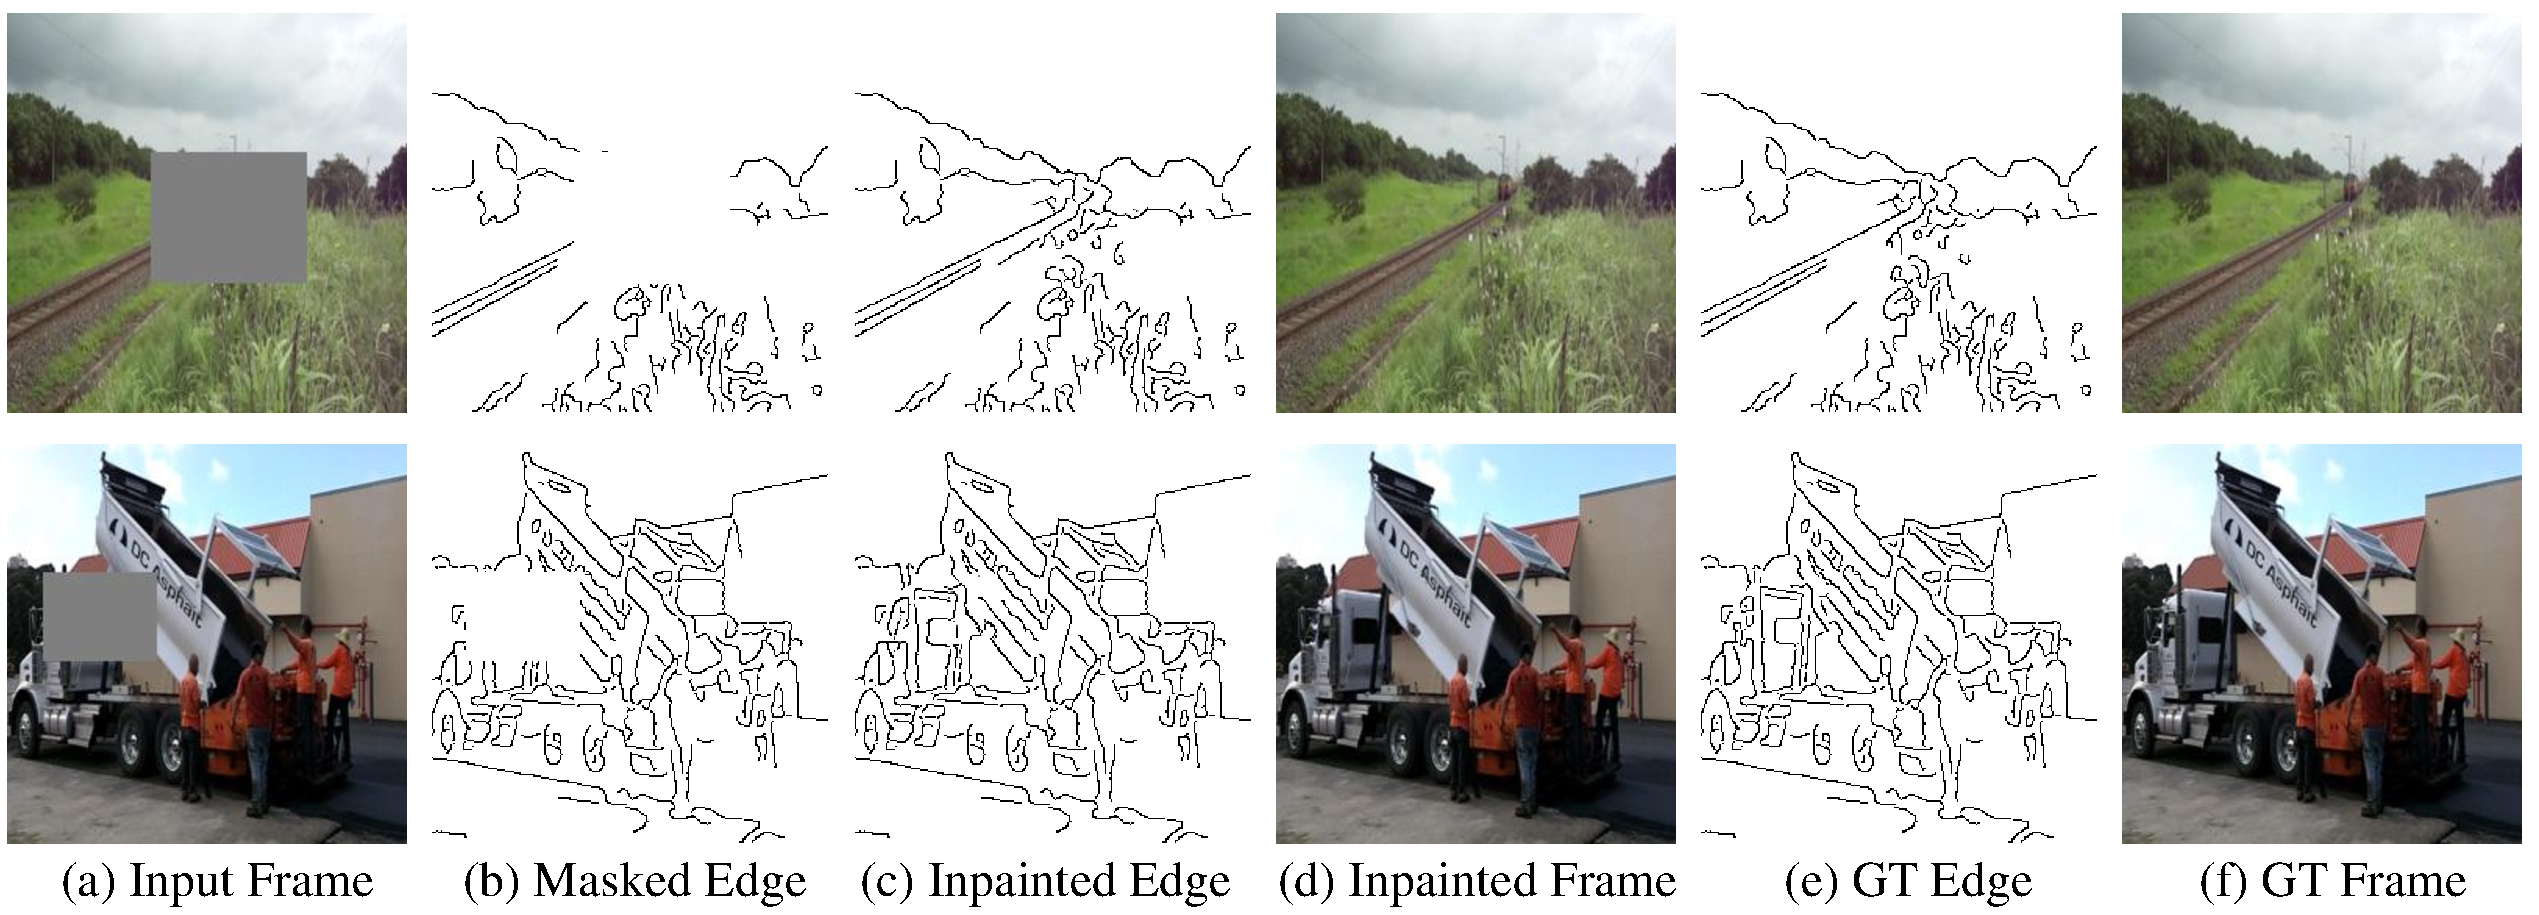
\includegraphics[width=0.97\columnwidth]{edgevis} % Reduce the figure size so that it is slightly narrower than the column. Don't use precise values for figure width.This setup will avoid overfull boxes. 
	\caption{Visualized effects of exploring structure edges in video inpainting. It's obvious that we can obtain more detail-clear results with structure guidance.}
	\label{edgevis}
\end{figure}
The quantitative results are shown in Table~\ref{tab:sem}. 
%As shown, the network achieves better results when edge information is utilized, comparing '+edge input' to 'STI'. It indicates that edge clues are effective guidance in video inpainting, which helps the network to predict more accurate frames.
We can see that '+edge input' brings large improvement over the baseline STI.
It indicates that the edge clues are effective guidance in video inpainting, which helps the network to predict accurate missing content.
When we further add SAM to STI, extra improvement is obtained.
It demonstrates that, compared with original edge, the latent structure information,~\emph{i.m.}~spatial correlation between structural edge and video texture, can be better embedded and absorbed by STI.
The above analyses prove that the edge clues are effective guidance in video inpainting, which helps the network to predict more accurate frames.

Furthermore, the visualized results are given in Fig.~\ref{edgevis}. It's obvious that after introducing the edge structure, the inpainted frames become visually better, with sharper object contours. Besides, the edge maps predicted by our method are reasonable and clear, which well represents the structure information and show the strong edge inpainting ability of ENet.
Thus, it is crucial to explore structural details when inpainting the videos.






\begin{figure}[t]
	\centering
	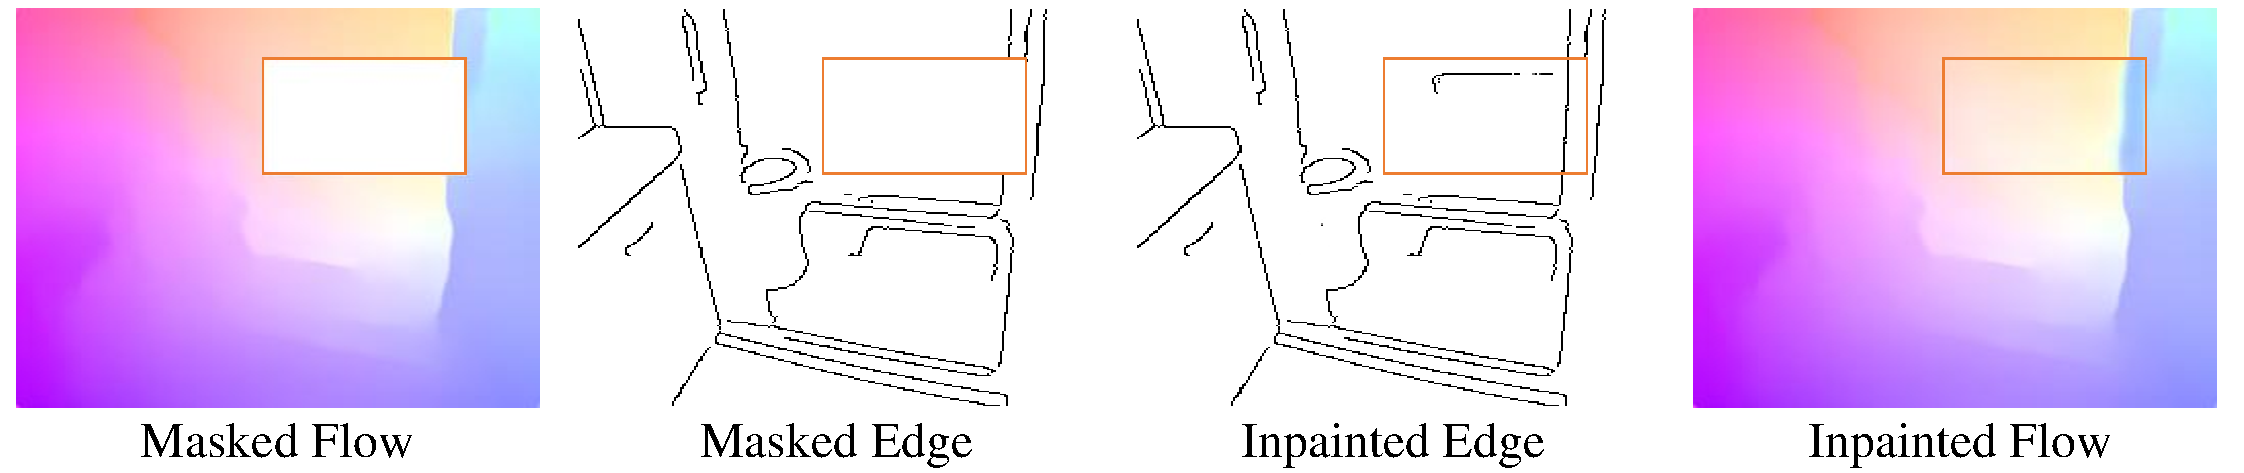
\includegraphics[width=1.0\columnwidth]{flowvis} % Reduce the figure size so that it is slightly narrower than the column. Don't use precise values for figure width.This setup will avoid overfull boxes. 
	\caption{Visualized optical flow predicted by our method.}
	\label{flowvis}
\end{figure}
\begin{figure}[t]
	\centering
	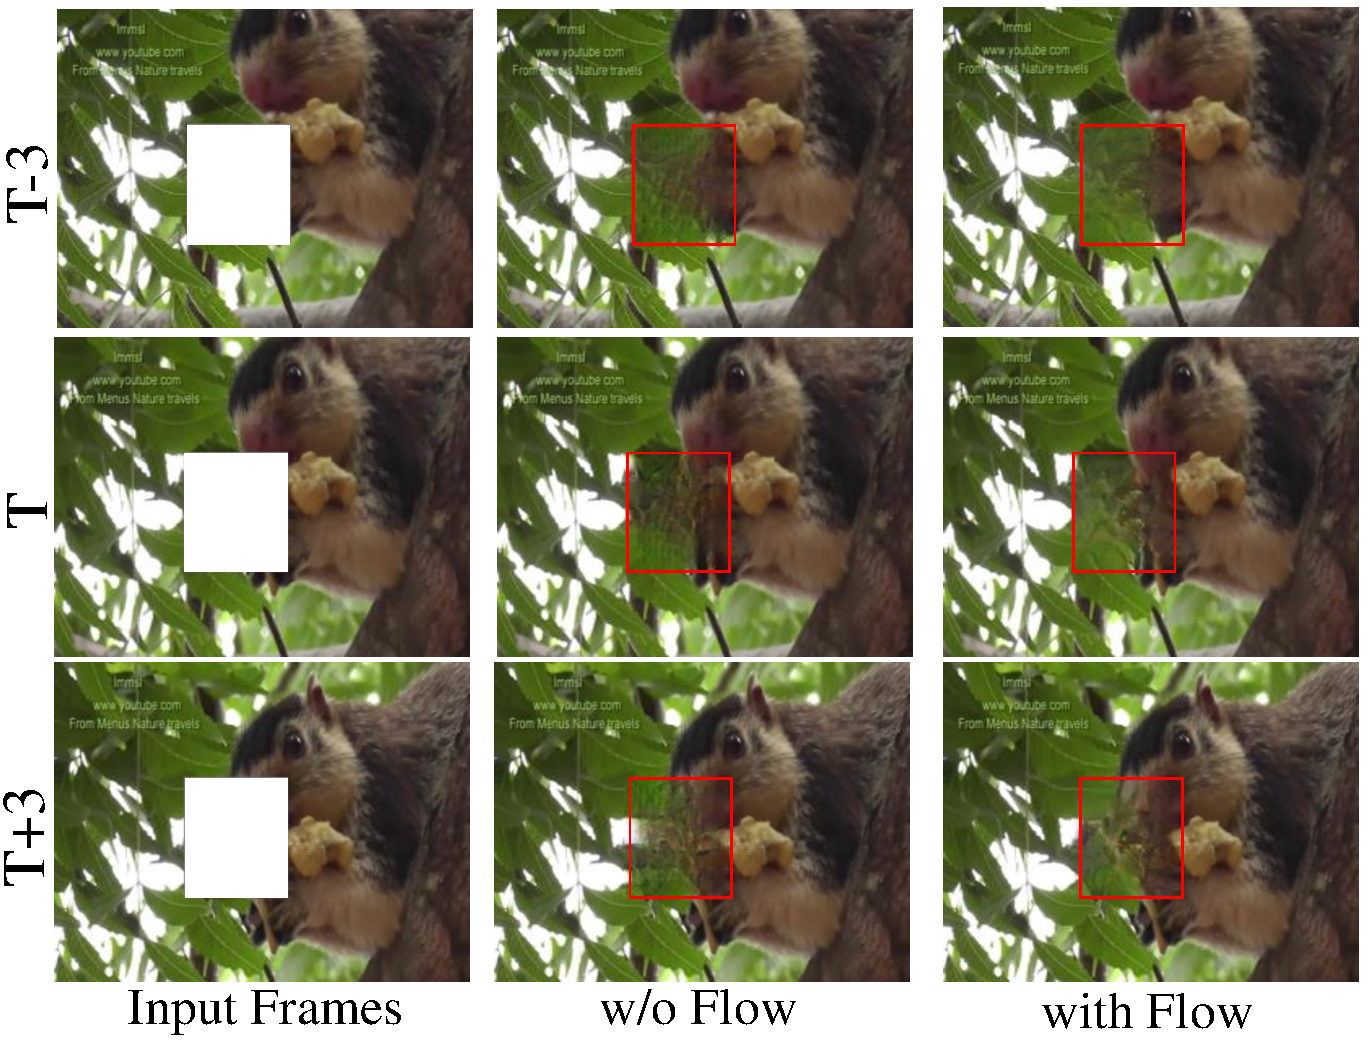
\includegraphics[width=1.0\columnwidth]{flow_vis} % Reduce the figure size so that it is slightly narrower than the column. Don't use precise values for figure width.This setup will avoid overfull boxes. 
	\caption{Visualized effects of temporal information.}
	\label{flow_vis}
\end{figure}

\subsubsection{Effect of Temporal Information in TINet.}
Temporal consistency is also an important factor in video inpainting. In our method, we utilize temporal information from the inpainted flows to smoothen the artificial flickers via the developed flow-guided warping and temporal ensemble module. 
%We use '+flow' to denotes the model 
First of all, we provide the visualized results in Fig.~\ref{flowvis}, where the proposed FNet can effectively complete the missing flows with fine boundaries.
Then, the quantitative results are given in Table~\ref{tab:sem}.
'Ours' is denoted as our model that utilizes flow-guided warping and temporal ensemble module.
It can be seen that the result is further improved after utilizing temporal information. It proves that the complementary contents can be aggregated by motion, which is helpful in video inpainting. 
As shown in Fig.~\ref{flow_vis}, the motion information can smoothen artificial flickers, resulting in temporal consistent inpainting results, and the color changes between neighboring frames become less obvious after employing flow.
Furthermore, it should be noted that the performance improvement from temporal information is smaller than that from structure information in this paper.
The reason maybe that our base model has certain ability to utilize complementary information of neighboring frames.
%a flow warping loss to smoothen the artificial flickers and propagate complementary information from neighboring frames. 
%It is achieved by $\mathcal{L}_{fec}$, which demonstrates that structure information can also boost the completion of optical flow.
%To evaluate the impact of temporal smoothening in STI, we compare two baselines, STI and STI w/o flow.
%As shown in Table~\ref{tab:edge}, STI works better than STI w/o flow, values...!!!.
%The visualized results are shown in Fig.~\ref{flow_vis}.
%It can be observed that the artificial flickers are alleviated when motion guidance is involved. 
Both the quantitative and qualitative results prove that the motion information is beneficial to temporal consistency as well as inpaitning.
%Besides, he visulization results in Fig.~\ref{flowvis} shows that $\mathcal{L}_{fec}$ encourages the network to predict optical flow  which demonstrates that structure information can also boost the completion of optical flow.

%We only use the first three mask settings on YouTubeVOS.
%\cxj{for what reason? page limit of the paper? How about others? Can we result in the same conclusion for different mask settings?}


%We discussed four variants of our method. We 
%\begin{enumerate}
%	\item STI: The Spatio-Temporal Inpainting network without guidance of either edge or flow.
%	\item +edge:
%	\item Free-from mask. We apply irregular mask which imitates hand-drawn masks on each frame, following \cite{liu2018partialinpainting}. 
%	\item Foreground object mask. This type of masks are defined to line out the foreground objects in videos, which is used for object removal.
%\end{enumerate}
%\noindent \textbf{Baselines.} Several variants of STSENet are defined as following. (1) STI w/o flow: The Spatio-Temporal Inpainting network without flow guidance \cxj{with or without EdgeNet and SEM?}. (2) STI w/o edge: The Spatio-Temporal Inpainting network without structure guidance. (3) STSENet w/o $\mathcal{L}_{fec}$: The Spatio-Temporal Inpainting network with guidance of both structure and motion, but $\mathcal{L}_{fec}$ is not used. (4) STSENet is the model which uses all modules proposed in this paper. 
%
%\cxj{We discussed four variants of our method. Use that version. }
\begin{figure}[!h]
	\centering
	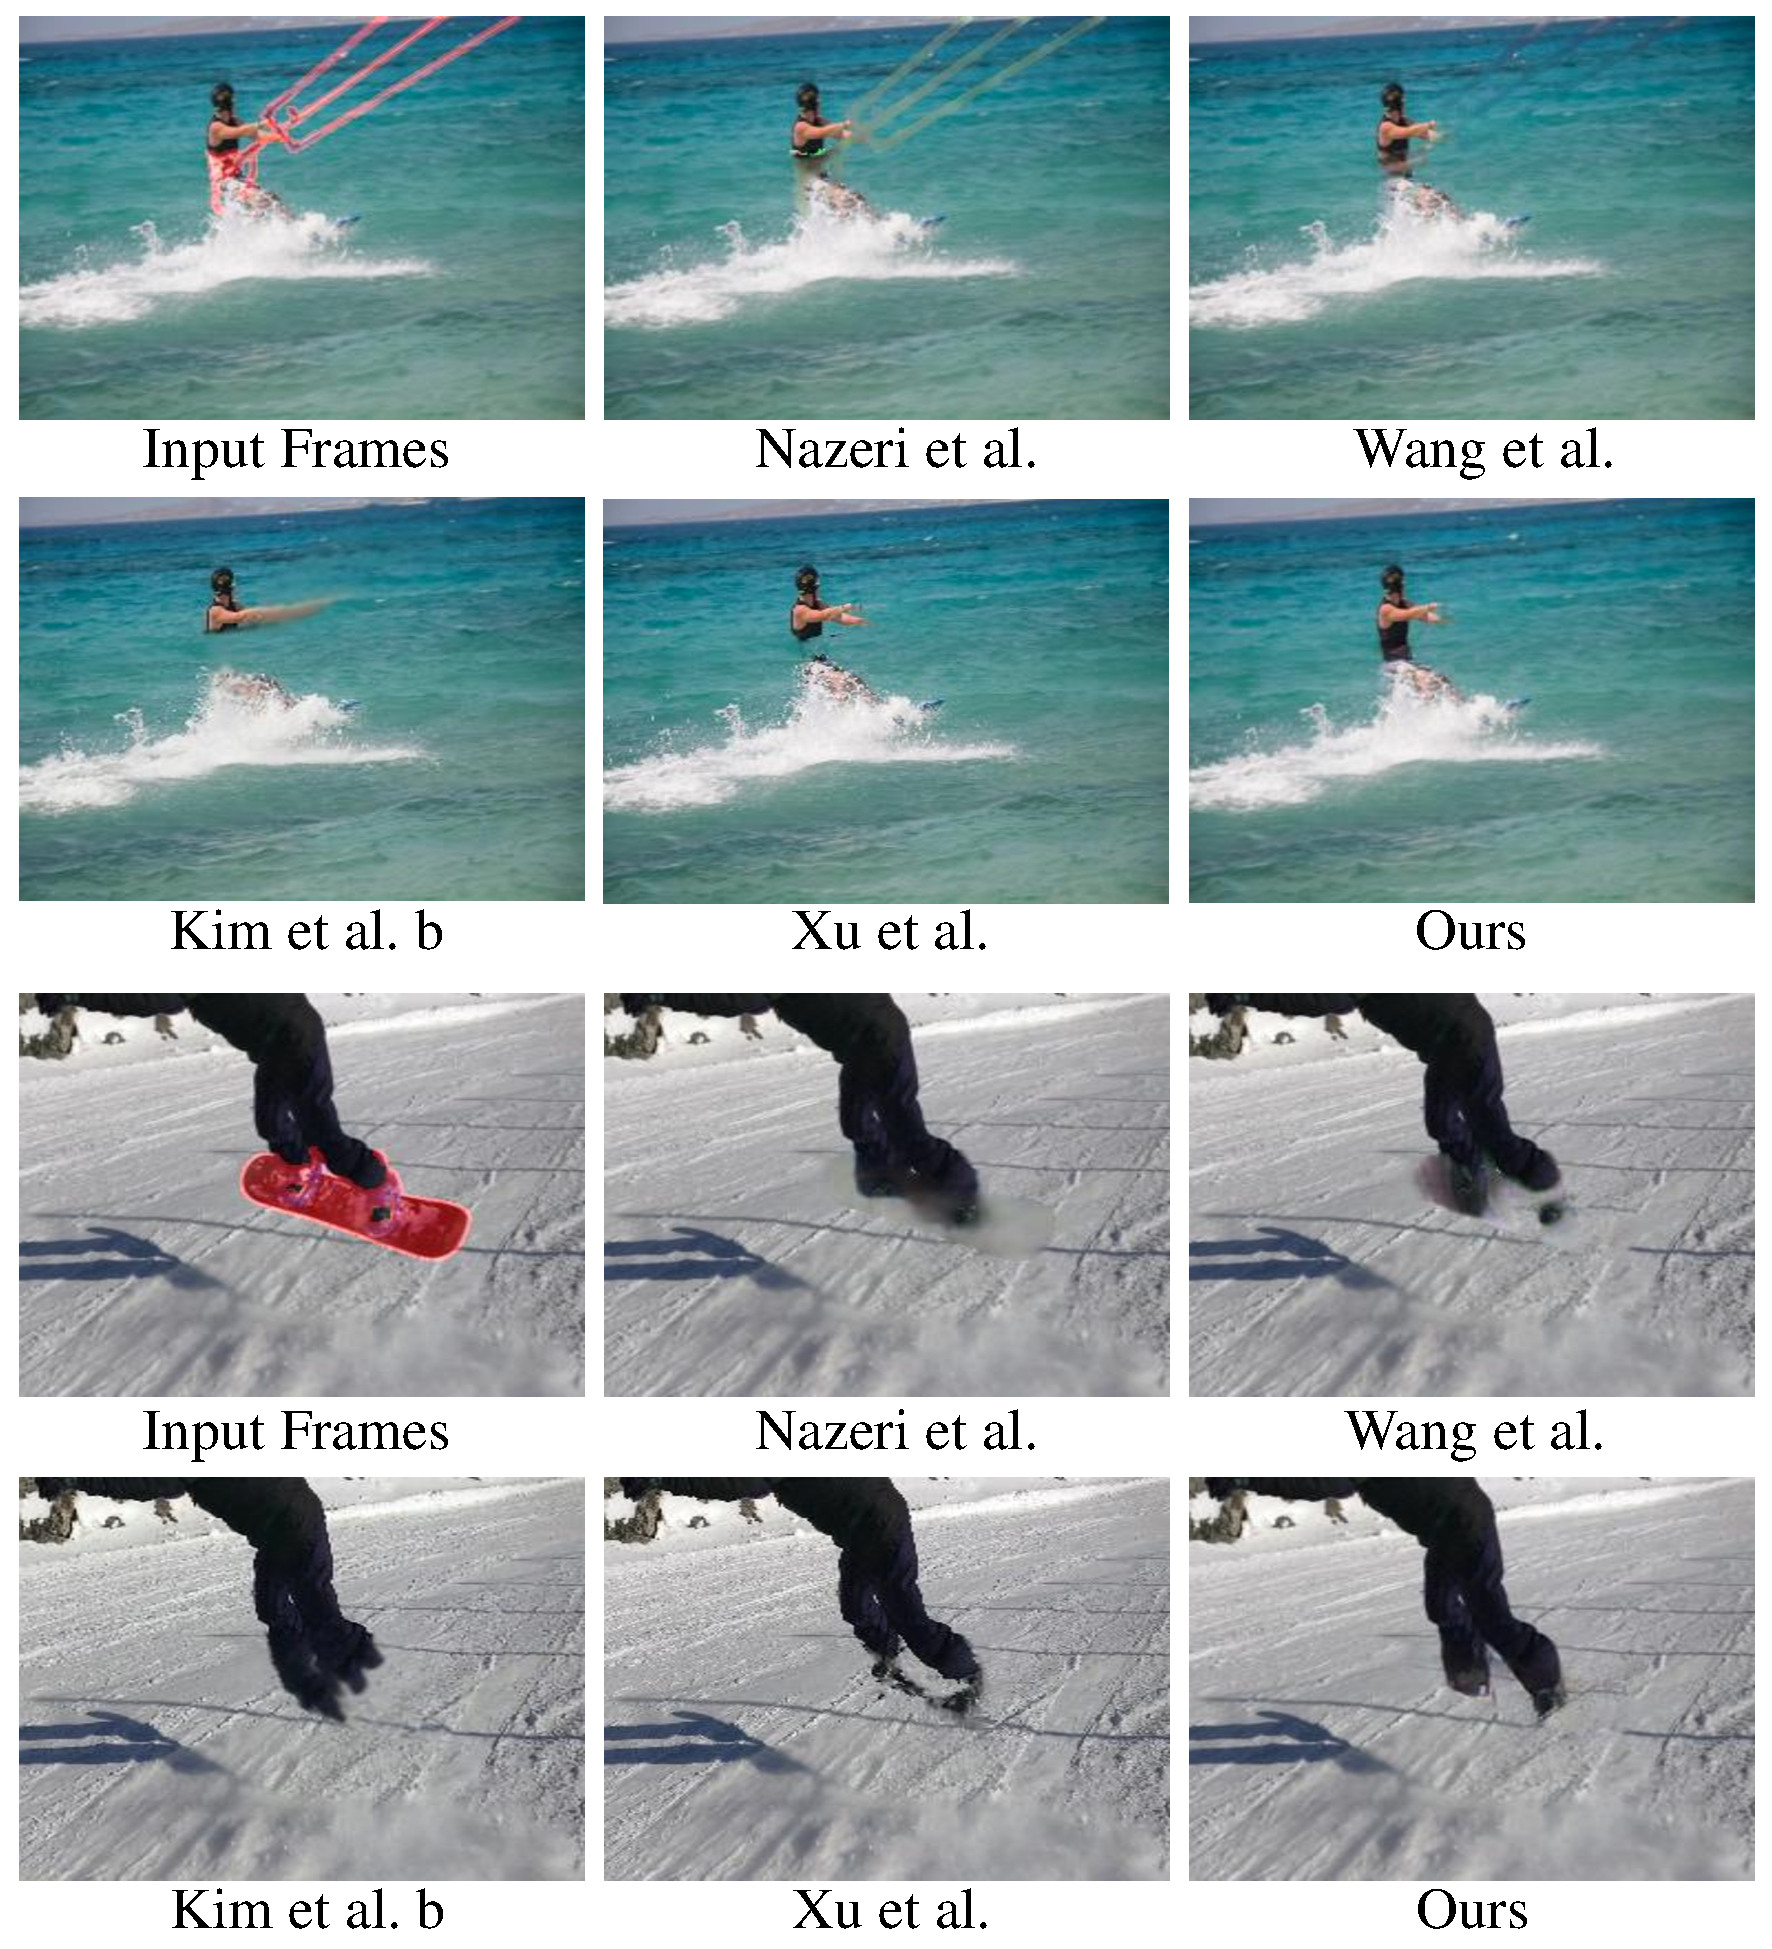
\includegraphics[width=1.0\columnwidth]{vis_forg} % Reduce the figure size so that it is slightly narrower than the column. Don't use precise values for figure width.This setup will avoid overfull boxes. 
	\caption{Visualized object foreground removal. The red mask in input frames indicates the object that we want to remove.}
	\label{vis_forg}
\end{figure}
\subsection{Comparisons with Existing Methods.}
We compare our results with state-of-the-art inpainting methods \cite{nazeri2019edgeconnect,wang2019video,Kim_2019_CVPR1,Xu_2019_CVPR}. 
As shown in Table~\ref{tab:sem}, Our structure-oriented method achieves better results than other methods, which demonstrates the effectiveness of introducing structural clues into video inpainting.
Specifically, the additional time cost brought by edge enhancement is negligible.
When the flow inpainting module is removed in SOVI, the inference speed is almost twice faster, and our performance is still competitive.
Notably, \cite{nazeri2019edgeconnect} is the image inpainting method which uses structure information. We surpass it by a large margin, which demonstrates that SOVI not a naive extension to utilize structure information in video inpainting.
This indicates that structure clues can bring strong promotion to video inpainting, 
We also give qualitative results in Fig.~\ref{viszong}. Compared with existing methods, inpainting results predicted by our method are more realistic with finer details. We can observe that the frames predicted by our method contain more sharper object contours. This is achieved by the effectiveness of structure information in video inpainting.









%\noindent \textbf{Effect of Flow-Edge Consistency Loss.}
%Flow-edge consistency loss $\mathcal{L}_{fec}$ is designed for mutual improvement of optical flow and edge maps.
%To demonstrate the effectiveness of $\mathcal{L}_{fec}$ in training, we compare the performances between STSENet w/o $\mathcal{L}_{fec}$ and STSENet. We use standard end-point-error (EPE) metric to evaluate the completion of optical flow. Besides, the well-completed flow and edge aid the final inpainting results, so the quality of final inpainting results also reflects the impact of $\mathcal{L}_{fec}$.
%The quantitative results are shown in Table~\ref{tab:lfec}. It indicates that $\mathcal{L}_{fec}$ plays a positive role in prediction of flow and edge, which is helpful for video inpainting. 
%\begin{table}[t]
%	\caption{The effect of structure clues and temporal smoothening in STSENet. The mask number denotes the indexes of mask setting in the section Experimental Settings. We compare STI,STI w/o SEM, and  in three aspects of metrics.}\smallskip
%	\centering
%	\resizebox{.95\columnwidth}{!}{
%		\smallskip\begin{tabular}{c|c|c|c|c|c|c|c|c|c }
%			\hline
%&\multicolumn{3}{c|}{Fixed Square}& \multicolumn{3}{c|}{Moving Square}&\multicolumn{3}{c}{Free-Form}\\
%\cline{2-10} 
%&PSNR & SSIM & FID & PSNR & SSIM & FID & PSNR & SSIM & FID\\
%\hline
%STI &28.0174 &0.9494  &  42.7164   &	
%33.8131 &  0.9705  &8.2390	& 
%30.0680& 0.9390 & 20.6358
%\\
%\hline
%+edge input  &29.5242 &  0.9520& 36.2097   &	
%37.6630	& 0.9798 &3.5161    &	
%33.8206	&0.9659  &    6.6651  \\
%\hline
%
%+SEM &29.9918 &  0.9533 &  27.4198  &	
%38.2433	& 0.9807 &   2.5083  &	
%35.7783	&0.9712  &   5.8786  \\
%\hline
%
%+flow &\textbf{30.0590} &\textbf{0.9543}&   \textbf{27.2431}  &
%\textbf{38.8186} & \textbf{0.9824} & \textbf{2.3455} &
%\textbf{35.9613}  & \textbf{0.9721}&  \textbf{ 5.8694} \\
%
%\hline
%			
%			
%		\end{tabular}
%	}
%	\label{tab:edge}
%\end{table}






\subsection{User Study on Video Object Removal}
Evaluation metrics can not fully reflect the quality of inpainted videos. So in addition to qualitative comparison, we also conduct a user study on DAVIS dataset to evaluate the visual quality of our method. We compare our method with the strong methods \cite{nazeri2019edgeconnect,wang2019video,Kim_2019_CVPR1,Xu_2019_CVPR}.
In each test, the origianl video, result produced by our method and result of another method are shown at the same time. The participants are allowed to play the videos multiple times to notice the differences of results of different methods.
we invite 30 participants for the user study. Each participant has to watch 20 random videos carefully, and choose which method is visually better. We list the preferred proportion of each methods compared to ours. The results are reported in Table~\ref{tab:userstudy}, which shows that our method is preferred by the users. Visualization in Fig.~\ref{vis_forg} also demonstrates that the results generated by our methods are visually better than existing methods.
\begin{table}[t]
	\caption{The result of user study.}\smallskip
	\tiny
	\centering
	\resizebox{0.7\columnwidth}{!}{
		\smallskip\begin{tabular}{c|c}
			\hline
			Comparing Methods&Preferred Proportion\\
			\hline
			Ours/Nazeri et al.&0.9083/0.0917\\
			\hline
			Ours/Wang et al. &0.8015/0.1985\\
			\hline
			Ours/Kim et al. b &0.7357/0.2643\\
			\hline
			Ours/Xu et al. &0.5941/0.4059\\
			\hline
			
			
		\end{tabular}
	}
	\label{tab:userstudy}
\end{table}






\section{Conclusion}
In this paper, we propose a novel structure-oriented video inpainting method, which utilizes sturcture information to generate fine-detailed frames. We first complete edge maps, which indicate structure details in frames. Then we generate frames under the guidance of structure information. Besides, we synthesize missing optical flow to constrain the temporal consistency of final outputs.
Experiments on YouTubeVOS and DAVIS datasets demonstrate the effectiveness of our method of utilizing structure preserving in video inpainting.


% Specifically, we jointly complete edge maps and optical flow with a consistency loss, which helps to obtain temporal consistent edge and edge-clear optical flow. Then with the guidance of spatial details and motion tendency, spatio-temporal inpainting network is designed to predict the final video with fine spatial details few artificial flickers.
%The state-of-the-art performance on both YouTube-VOS and DAVIS prove the effectiveness of exploring structural clues and optical flow in video inpainting.

